\chapter{عنوان فصل یا پیوست}

به‌عنوان مثال مقداری متن در این قسمت قرار می‌دهیم. فرض کنید $\mathbb{K}$ یک میدان و $S=\mathbb{K}[x_1, \ldots, x_n]$ حلقه چندجمله‌ای‌ها روی میدان $\mathbb{K}$ باشد که با درجه‌بندی استاندارد مدرج شده است. فرض کنید $M = \oplus_{i\in \mathbb{Z}}M_i$ یک $S$-مدول ناصفر با تولید متناهی باشد. به ازای هر $i \in \mathbb{N} \cup \{0\}$، تعریف می‌کنیم:
\[t^S_i(M) = \max \{j \colon \quad \beta^\mathbb{K}_{i,j}(M) \neq 0\} \]
که در آن $\beta^\mathbb{K}_{i,j}(M)$، همان $i,j$-امین عدد بتی $M$ به عنوان $S$-مدول است. در واقع
\[\beta^\mathbb{K}_{i,j}(M) = \dim_\mathbb{\mathbb{K}} \mathrm{Tor}_{i}^{S}(\mathbb{\mathbb{K}},M)_j\]
در حالتی که $\mathrm{Tor}_{i}^{S}(\mathbb{\mathbb{K}},M)=0$، قرار می‌دهیم $t^S_i(M)= - \infty$.

عدد نظم کاستلنوو-مامفورد $M$ که با $\mathrm{reg}(M)$ نمایش  می‌دهیم را به صورت زیر تعریف  می‌کنیم:
\[\mathrm{reg} (M)= \sup \{t^S_i(M)-i \colon \quad i \in \mathbb{Z} \}.\]

همچنین درجه آغازین یک $S$-مدول با تولید متناهی و ناصفر $M= \oplus_{i\in \mathbb{Z}}M_i$ را با $\mathrm{indeg}\, (M)$ نمایش داده و به صورت زیر تعریف  می‌کنیم:
\[\mathrm{indeg}\, (M)=\inf \{i \colon \quad M_i \neq 0 \}.\]
گوییم $M$ دارای تحلیل $d$-خطی است، هرگاه 
$\mathrm{reg}(M)=\mathrm{indeg}\,(M)$.

\begin{theorem} 
فرض کنید $M \neq 0$ یک $S$-مدول با تولید متناهی باشد. موارد زیر هم‌ارز هستند:
\begin{itemize}
\item[(آ)] $a = \mathrm{reg} (M)$.
\item[(ب)] $a = \max\{t \colon \quad \beta^\mathbb{\mathbb{K}}_{i,i+t}(M) \neq 0; \quad i \geq 0 \text{به‌ازای برخی } \}$.
\item[(پ)] $a = \max \{t \colon \quad \mathrm{Tor}_{i}^{S}(K,M)_{t+i} \neq 0; \quad i \geq 0 \text{به‌ازای برخی } \}$.
\item[(ت)] $a = \max \{t \colon \quad \mathrm{Ext}_{S}^{i}(K,M)_{-t-i} \neq 0; \quad i \geq 0 \text{به‌ازای برخی } \}$.
\item[(ث)] $a = \max \{t \colon \quad  {H_\mathfrak{m}^i(M)}_{t-i} \neq 0; \quad i \geq 0 \text{به‌ازای برخی } \}$.
\item[(ج)] $a = \max \{a_i(M)+i \colon \quad i \in \mathbb{N} \}$ که در آن  $a_i(M)= \max \{t \colon \quad {H_\mathfrak{m}^i (M)}_{t} \neq 0 \}$.
\end{itemize}
\end{theorem}

\section{عنوان بخش }
متن بخش اول را در اینجا بنویسید.
\begin{definition}
فرض کنید $[n]=\{1, \ldots,n\}$ و $\Delta$ یک مجتمع سادکی بر $[n]$ باشد. دراین‌صورت ایدآل استنلی-رایزنر $\Delta$ را با $I_\Delta$ نمایش داده و به‌صورت زیر تعریف می کنیم
\[I_\Delta=(\mathbf{x}_F \colon \quad F \notin \Delta).\]
\end{definition}

\subsection{عنوان زیر بخش }

\begin{theorem}\label{Resolution of minimal}
فرض کنید $\mathcal{C}$ یک $d$-ابرگراف روی مجموعه رأس‌های $[n]$ باشد که مینیمال نسبت به $d$-خطی‌بودن است و 
 $I=I(\bar{\mathcal{C}}) \subset \mathbb{K}[x_1, \ldots, x_n]$ 
  ایدآل متناظر با 
 $\mathcal{C}$
  باشد. در این‌صورت تحلیل آزاد مینیمال ایده‌آل
  $I$
   به صورت زیر است:
\begin{align*} 
0  \to S^{\beta_{n-d,n}}(-n) & \to S(-n) \oplus S^{\beta_{n-d-1, n-1}}(-(n-1)) \to  S^{\beta_{n-d-2, n-2}}(-(n-2))  \\
& \to \cdots \to S^{\beta_{1,d+1}}(-(d+1)) \to S^{\beta_{0,d}}(-d) \to I \to 0 \label{Resolution of Minimal to linearity+Shape}
\end{align*}
که در آن،
\begin{itemize}
\item[(آ)] 
$\beta_{n-d,n}(I) = 1 -e(S/I) + \sum\limits_{i=0}^{d-1} (-1)^{d+i-1} {n \choose i}$.
\item[(ب)]
برای $0 \leq i \leq n-d-1$، داریم 
$\beta_{i, i+d}(I) = {n-d \choose i} \left( \frac{d}{d+i}{n \choose d} - e(S/I) \right)$.
\end{itemize}

\end{theorem}

\begin{example}[رجوع شود به {\cite[{قضیه 5.3}]{Morales_Pour_Zaare-Nahandi_2016}}]
فرض کنید $\Delta$ یک مثلث‌بندی از کره $\mathbb{S}^2$ با $n>4$ رأس باشد و $\mathcal{C}=\mathcal{F}(\Delta)$، ابرگراف متناظر با $\Delta$ باشد. دراین‌صورت $\mathcal{C}$ یک $3$-شبه‌منیفلد جهت‌پذیر است. پس با توجه به قضیه، ابرگراف $\mathcal{C}$ مینیمال نسبت به $3$-خطی‌بودن است. لذا قضیه \ref{Resolution of minimal} ایجاب می‌کند که تحلیل آزاد مینیمال ایدآل   $I=I(\bar{\mathcal{C}})$  به صورت زیر است:
\begin{align*} 
0 \to S^{\beta_{n-3,n}}(-n) \to S(-n) \oplus S^{\beta_{n-4, n-1}}(-(n-1)) \to  S^{\beta_{n-5, n-2}}(-(n-2)) \\
 \to \cdots \to S^{\beta_{0,3}}(-3) \to I \to 0
\end{align*}
که در آن،
\[\beta^\mathbb{K}_{i, i+3}(I) = {n-3 \choose i} \left( \frac{3}{3+i}{n \choose 3} - 2(n-2) \right).\]

\end{example}
\section{بخش دوم}
\begin{proposition}
مقداری متن مقداری متن مقداری متن مقداری متن مقداری متن 
\end{proposition}



\begin{corollary}
مقداری متن مقداری متن مقداری متن مقداری متن مقداری متن 
\end{corollary}



\begin{lemma}
مقداری متن مقداری متن مقداری متن مقداری متن مقداری متن 
\end{lemma}



\begin{conjecture}
مقداری متن مقداری متن مقداری متن مقداری متن مقداری متن 
\end{conjecture}


\begin{remark}
مقداری متن مقداری متن مقداری متن مقداری متن مقداری متن 
\end{remark}


\begin{question}
مقداری متن مقداری متن مقداری متن مقداری متن مقداری متن 
\end{question}


\begin{problem}
مقداری متن مقداری متن مقداری متن مقداری متن مقداری متن 
\end{problem}


\begin{notation}
مقداری متن مقداری متن مقداری متن مقداری متن مقداری متن 
\end{notation}




\begin{figure}[h]
\centering
\begin{tabular}{ccc}
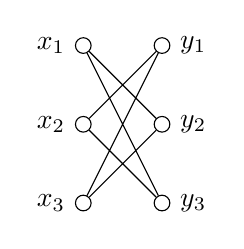
\begin{tikzpicture}
\node [draw, fill=white, circle, inner sep=2pt, label=left:{$x_3$}] (x3) at (0,0) {};
\node [draw, fill=white, circle, inner sep=2pt, label=left:{$x_2$}] (x2) at (0,1) {};
\node [draw, fill=white, circle, inner sep=2pt, label=left:{$x_1$}] (x1) at (0,2) {};
\node [draw, fill=white, circle, inner sep=2pt, label=right:{$y_3$}] (y3) at (1,0) {};
\node [draw, fill=white, circle, inner sep=2pt, label=right:{$y_2$}] (y2) at (1,1) {};
\node [draw, fill=white, circle, inner sep=2pt, label=right:{$y_1$}] (y1) at (1,2) {};

\draw (x1)--(y2)--(x3)--(y1)--(x2)--(y3)--(x1);
\end{tikzpicture}
&\ \hspace{2cm}\ &
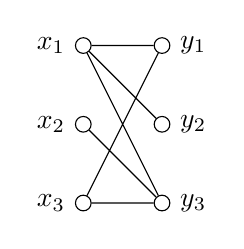
\begin{tikzpicture}
\node [draw, fill=white, circle, inner sep=2pt, label=left:{$x_3$}] (x3) at (0,0) {};
\node [draw, fill=white, circle, inner sep=2pt, label=left:{$x_2$}] (x2) at (0,1) {};
\node [draw, fill=white, circle, inner sep=2pt, label=left:{$x_1$}] (x1) at (0,2) {};
\node [draw, fill=white, circle, inner sep=2pt, label=right:{$y_3$}] (y3) at (1,0) {};
\node [draw, fill=white, circle, inner sep=2pt, label=right:{$y_2$}] (y2) at (1,1) {};
\node [draw, fill=white, circle, inner sep=2pt, label=right:{$y_1$}] (y1) at (1,2) {};

\draw (y2)--(x1)--(y1)--(x3)--(y3)--(x1) (x2)--(y3);
\end{tikzpicture}\\
\end{tabular}
\caption{دو مثال از گراف‌های دوبخشی}
\label{figure: bipartite graph}
\end{figure}


\begin{latin}
\begin{algorithm}[H]
\begin{algorithmic}[1]\baselineskip=10pt\relax

\REQUIRE A labeled bipartite graph $ \Gamma $ with bipartition $ X, Y $
\ENSURE A positive matching decomposition of $ \Gamma $
\STATE $ k\longleftarrow 0 $
\WHILE{$ E(\Gamma) \neq \varnothing $}
\STATE $ k \longleftarrow k + 1 $
\STATE  $ X' \longleftarrow X \setminus \{\text{isolated vertices of } X\}$
\STATE  $ Y' \longleftarrow \varnothing $
\STATE $M_k \longleftarrow \varnothing $
\WHILE{$ X' \neq \varnothing$}
\STATE $ s \longleftarrow \min(\text{Slopes}(\Gamma[X'\cup Y])) $
\STATE $ M \longleftarrow \{xy \in E(\Gamma[X'\cup Y]) \colon \quad \mathrm{slope}(xy)=s\} $
\STATE $ M_k \longleftarrow M_k \cup \{xy \in M \colon \quad y \notin Y'\} $
\STATE $ X' \longleftarrow X' \setminus \{x \colon \quad xy\in M\} $
\STATE $ Y' \longleftarrow Y' \cup \{y \colon \quad xy\in M\} $
\ENDWHILE
\STATE $E(\Gamma) \longleftarrow E(\Gamma) \setminus M_k $
\ENDWHILE
\RETURN $ M_1,\ldots,M_k$

\end{algorithmic}
\caption{\textsc{A positive matching decomposition of a labeled bipartite graph}}
\label{alg:A positive matching decomposition of a labeled bipartite graph}
\end{algorithm}
\end{latin}

\begin{latin}
\begin{table}[H]
\begin{tabular}{|c|c|c|>{\centering}p{3cm}|>{\centering}p{4cm}|}
\cline{3-5}
\multicolumn{2}{c}{} & \multicolumn{2}{|c|}{Oriented surfaces} & {Non-oriented surfaces} \tabularnewline
\cline{2-5}
\multicolumn{1}{c|}{} & {\multirow{2}{*}{$S$}} & {\multirow{2}{*}{Sphere}} & Connected sum of {$r$ tori} & Connected sum of $r$ Projective Plane \tabularnewline
%\multicolumn{1}{c|}{} &  &  & {$r$ tori} & $r$ Projective Plane \\
\cline{2-5}
\multicolumn{1}{c|}{} & $\chi(S)$ & $2$ & $2-2r$ & $ 2-r $ \tabularnewline
\hline
{\multirow{3}{*}{$\tilde{H}_i(S,\mathbb{K})$}} & $i=0$ & $0$ & $0$ & $0$ \tabularnewline
\cline{2-5}
 & $i=1$ & $0$ & $\mathbb{K}^{2r}$ & $(\mathbb{Z}_2 \otimes_\mathbb{Z} \mathbb{K}) \oplus \mathbb{K}^{r-1}$ \bigstrut\tabularnewline
\cline{2-5}
 & $i=2$ & $\mathbb{K}$ & $\mathbb{K}$ & $\mathrm{Tor}_{1}^{\mathbb{Z}}(\mathbb{Z}_2,\mathbb{K})$ \bigstrut\tabularnewline
\hline
\end{tabular}
\caption{Homology of $2$-manifolds}
\label{Table of Homology}
\end{table}
\end{latin}